\section{Illustrative implementation on sparse surveillance counts}
\label{s:application}

\begin{figure}[!t]
\centering
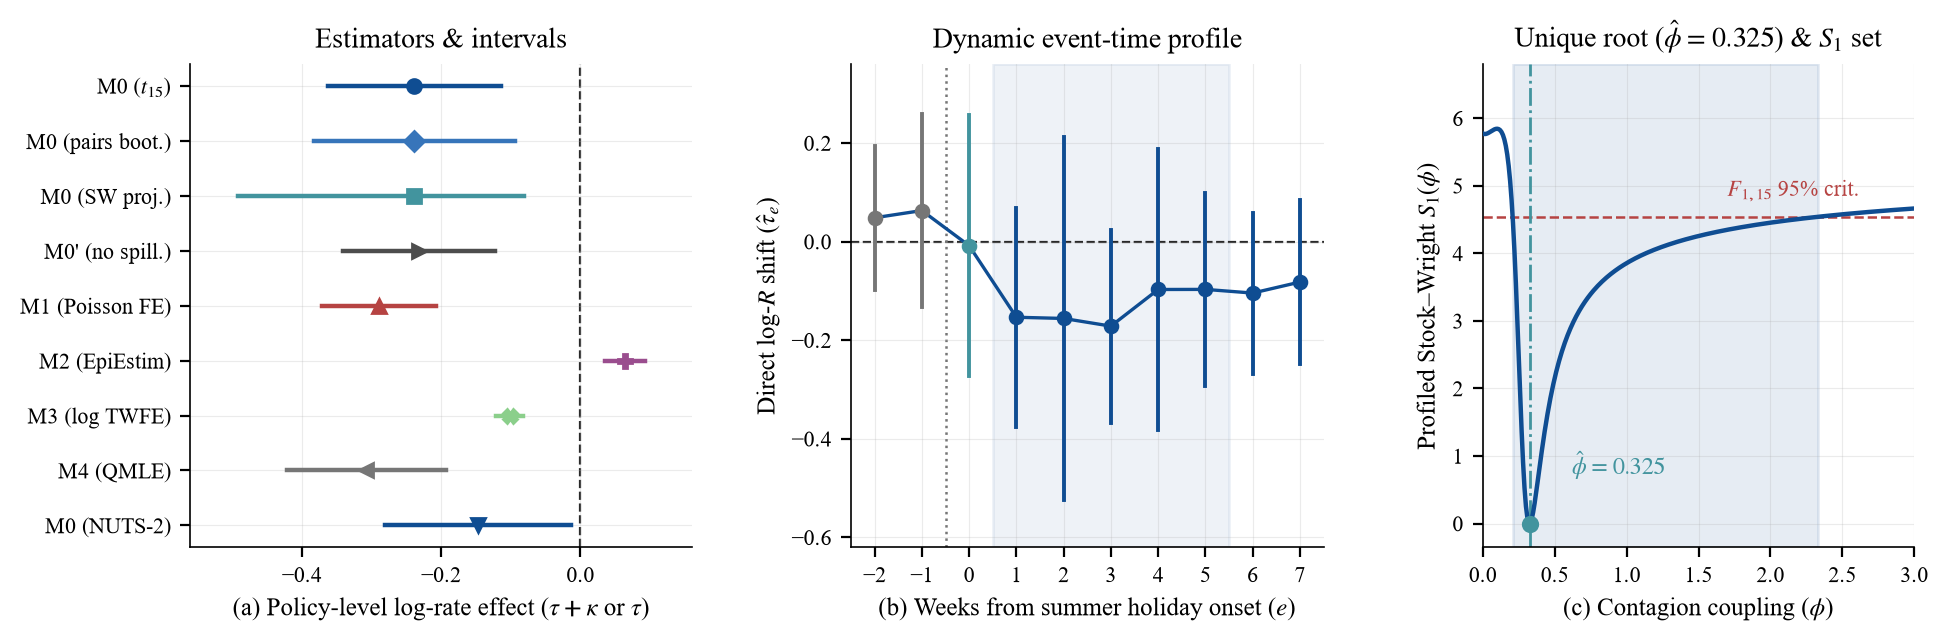
\includegraphics[width=\linewidth]{figures/fig_03_application.png}
\caption{Illustrative implementation on German county-level varicella notifications (2015--2019, $N=400$, $G=16$ federal states, $T=261$ weeks). (a) Working-model log-rate coefficient ($\hat\tau+\hat\kappa$, or $\hat\tau$) and 95\% intervals across QD-GMM M0 ($t_{15}$, WCR-score Webb6, and pairs cluster bootstrap-$t$), comparators (M0$'$, M1--M4), and NUTS-2 aggregation ($N=38$, reducing zero county-weeks from 58.8\% to 2.9\% and reversing two-step EpiEstim M2 from $+0.064$ to $-0.102$). (b) Profiled Stock--Wright $S_1(\phi)$ curve over $\phi\in[0,3]$ with boundary inset, showing local interior root $\hat\phi=0.326$ and exact-moment $F_{1,15}$ set $[0.21,2.40]$ (shaded).}
\label{fig:app}
\end{figure}

To demonstrate computation, comparator behaviour under extreme sparsity, and finite-cluster
calibration in real epidemic surveillance data, we implement QD-GMM on five years of weekly German
county-level varicella (\emph{Windpocken}) notifications paired with federal-state summer school
holidays (2015--2019; \citealp{faensen2006survnet}). Staggered German summer breaks have been used
in prior quasi-experimental analyses of school closures and respiratory pathogens
\citep{cauchemez2008school,jackson2014varicella,isphording2021schools,vonbismarckosten2022schools},
while \citet{adda2016economic} studied French weekly varicella incidence across school closures on
the outcome scale rather than the transmission scale. Here this panel serves as a computational and
diagnostic testbed in three respects. First, \citet{vink2014serial} report a mean varicella serial
interval of roughly 14.0 days; discretising a log-normal working surrogate with those moments onto
weekly lags $s=1,2,3$ gives $w=(0.141,0.720,0.138)$ with negligible within-week mass
($w_0=2.6\times 10^{-6}$, while serial and generation intervals share similar means but differ in
dispersion). Second, county-week notifications are sparse (58.8\% zeros, median 0, mean 1.10),
testing small-count comparator behaviour. Third, cluster sizes vary sharply across Germany's $G=16$
states (1 county in Berlin and Hamburg to 96 in Bavaria; median 16.5), providing a realistic
few-cluster setting.

\subsection{Data and working-model implementation}
\label{ss:app-data}

Weekly notified counts come from the Robert Koch Institute SurvStat@RKI 2.0 database (extracted
2026-11-19) for all $N=400$ German counties (merging Berlin's 12 districts into unit
\texttt{11000}, with zero imputed populations) over $T=261$ estimation weeks (2015-W01 through
2019-W52, 115{,}129 notifications, plus $S=3$ pre-sample weeks; Web Appendix~\ref{app:data}).
Official state summer holiday schedules come from OpenHolidays, and county adjacency comes from
five-digit AGS polygons (1{,}043 undirected edges, mean degree 5.22, row-normalised $W$). Given
varicella's approximately two-week serial interval and weekly \emph{Meldewoche} aggregation, the
baseline working exposure $D_{it}$ codes a one-week-lagged indicator for a majority of summer
holiday days ($\ge 4$ of 7 days) in state $g(i)$ (11.8\% of county-weeks); lag-2 sensitivity and
other calendar alignments are checked in Web Appendix~\ref{app:diag}. Background importation uses
$\omega_i=\text{population}_i/10^5$, and inference clusters by state ($G=16$). Because exposure
varies at the state level, interior counties satisfy $D_{it}=\bar D_{it}$, making $\tau+\kappa$ the
baseline working-model coefficient.

Without dropping any zero-count county-weeks, local QD-GMM M0 ($\bar\phi=0.5$) converges to a
single interior root $\hat\phi=0.326$ (SE $0.0567$, 95\% $t_{15}$ CI $[0.205,0.446]$;
Figure~\ref{fig:app}(b)), with baseline working-model coefficients $\hat\tau=-0.300$ ($[-0.854,0.254]$),
$\hat\kappa=0.060$ ($[-0.538,0.659]$), and $\hat\tau+\hat\kappa=-0.239$ (SE $0.0584$, 95\% $t_{15}$
CI $[-0.364,-0.115]$; Table~\ref{tab:app}). The numerical value $\hat\tau+\hat\kappa=-0.239$ is
reported strictly as a working-model implementation output and is not interpreted as a causal
school-holiday effect. Moreover, the single interior root is qualified by the broader root and
over-identification diagnostics: under exact working moments $S_1(0)=5.78$ ($p_F=0.030$) and the
95\% $S_1(F)$ set is $[0.21,2.40]$, yet the pre-specified global rule M0-G selects the $\phi=0$
boundary ($\hat\tau+\hat\kappa=-0.215$, Table~\ref{tab:app}) because $S_{3,\mathrm{oi}}$ slightly
favours $\phi=0$ over the interior root ($9.113$ vs.\ $9.120$), and M0-GI retains the interior root
only under $S_{3,\mathrm{inv}}$.

\subsection{Sparse-count estimator comparison}
\label{ss:app-comp}

On the observed surveillance panel, standard comparators exhibit patterns consistent with the
small-count distortions in Theorem~\ref{thm:bias} (Table~\ref{tab:app}, Figure~\ref{fig:app}(a)).
At the county level (58.8\% zeros), two-step EpiEstim log-$R$ DiD (M2) yields $+0.064$
($[0.036,0.093]$); aggregating identical counts into Germany's $N=38$ NUTS-2 regions lowers zeros
to 2.9\%, moving M2 immediately to $-0.102$ ($[-0.150,-0.055]$) while M0 moves from $-0.239$ to
$-0.147$ ($[-0.280,-0.013]$), $\log(Y+1)$ TWFE (M3) gives $-0.102$, and Poisson fixed effects (M1)
and pooled QMLE (M4) estimate near-zero spatial coupling ($0.058$ and $0.001$). Because M0 itself
shifts across observed aggregation levels, Web Table~\ref{tab:rev-calsim}(c) directly evaluates M2
and M3 against known generating truth ($\tau+\kappa=-0.239$) in the design-calibrated simulation
(Section~\ref{ss:app-wcr}): under simulated county zero shares (54.5\% calibrated, 57.8\%
high-noise), county M0 bias is $-0.003$ ($-0.016$ high-noise) whereas county M2 suffers a bias of
$+0.224$ ($+0.227$ high-noise), flipping positive in 22.8\% (32.6\%) of draws; aggregating simulated
panels to NUTS-2 (2.3\%--3.6\% zeros) cuts M2's bias by two-thirds to $+0.076$ ($+0.083$) while
NUTS-2 M0 bias remains small ($+0.013$ calibrated, $-0.008$ high-noise).

\begin{table}[!t]
\centering
\caption{Illustrative estimator comparison in a sparse surveillance panel (German varicella, 2015--2019; $N=400$ counties, $G=16$ states, $T=261$ weeks).}
\label{tab:app}
\footnotesize
\setlength{\tabcolsep}{3.5pt}
\begin{adjustbox}{max width=\linewidth}
\begin{tabular}{llrrrr}
\toprule
sample & method & $\hat\tau+\hat\kappa$ (95\% CI) & $\hat\tau$ (95\% CI) & $\hat\kappa$ (95\% CI) & $\hat\phi$ (95\% CI) \\
\midrule
Primary (58.8\% zeros) & M0 & -0.239 (-0.364, -0.115) & -0.300 (-0.854, 0.254) & 0.060 (-0.538, 0.659) & 0.326 (0.205, 0.446) \\
Primary (58.8\% zeros) & M0-G & -0.215 (-0.330, -0.101) & -0.294 (-0.858, 0.270) & 0.079 (-0.527, 0.685) & 0.000 (boundary) \\
Primary (58.8\% zeros) & M0-GI & -0.239 (-0.364, -0.115) & -0.300 (-0.854, 0.254) & 0.060 (-0.538, 0.659) & 0.326 (0.205, 0.446) \\
Primary (58.8\% zeros) & M0$'$ & -- & -0.233 (-0.343, -0.124) & -- & -- \\
Primary (58.8\% zeros) & M1 (Poisson FE) & -0.290 (-0.372, -0.208) & -0.324 (-0.543, -0.105) & 0.034 (-0.195, 0.263) & 0.058 (0.026, 0.090) \\
Primary (58.8\% zeros) & M2 (EpiEstim $\log R$) & -- & 0.064 (0.036, 0.093) & -- & -- \\
Primary (58.8\% zeros) & M3 ($\log(Y+1)$ TWFE) & -- & -0.102 (-0.120, -0.083) & -- & -- \\
Primary (58.8\% zeros) & M4 (Pooled QMLE) & -0.307 (-0.422, -0.193) & -0.261 (-0.426, -0.095) & -0.047 (-0.236, 0.142) & 0.001 (-0.046, 0.049) \\
NUTS-2 (2.9\% zeros) & M0 & -0.147 (-0.280, -0.013) & -0.309 (-0.617, -0.001) & 0.162 (-0.220, 0.544) & 0.400 (-0.005, 0.805) \\
NUTS-2 (2.9\% zeros) & M2 (EpiEstim $\log R$) & -- & -0.102 (-0.150, -0.055) & -- & -- \\
\bottomrule
\end{tabular}
\end{adjustbox}
\par\smallskip\parbox{\linewidth}{\scriptsize Weekly RKI SurvStat varicella notifications across 400 German counties in $G = 16$ federal states, 261 estimation weeks (ISO 2015-W01 to 2019-W52, 115{,}129 notifications, plus three pre-sample lag weeks); $D$ = one-week-lagged state summer holiday indicator; $w = (0.141, 0.720, 0.138)$ ($w_0 = 2.6 \times 10^{-6}$). Working-model finite-cluster 95\% intervals for M0 $\tau+\kappa$: WCR-score Webb6 $[-0.419, -0.139]$; WCR-score Rademacher $[-0.429, -0.119]$; unrestricted score wild (Mammen) $[-0.358, -0.121]$; pairs cluster bootstrap-$t$ (999/999 converged) $[-0.385, -0.094]$; delete-one-state jackknife $[-0.375, -0.104]$; Stock--Wright Bonferroni projection $[-0.493, -0.081]$. These working-model contrasts illustrate estimation, small-count sign reversal in M2 ($+0.064$ to $-0.102$), and finite-cluster calibration rather than causal holiday effects; full calendar, placebo, over-identification, and seasonal diagnostics appear in Web Appendices~D--F.}
\end{table}


\subsection{Finite-cluster calibration}
\label{ss:app-wcr}

Because $G=16$ states span 1 to 96 counties (Bavaria holds 24\% of all counties), we evaluate
finite-cluster interval coverage in simulations calibrated to the exact 400-county, 261-week
German design ($R=500$ draws each in baseline-noise and high-noise arms, coverage MCSE
$\approx 0.010$; Web Appendix~\ref{app:fewcluster}, Web Table~\ref{tab:rev-calsim}). Across all
1{,}000 simulated panels, QD-GMM achieves 100\% unique interior convergence with negligible bias on
$\tau+\kappa$ ($-0.003$ calibrated), yet conventional state-clustered $t_{15}$ intervals undercover at
$0.902$ ($0.904$ high-noise) because sandwich SEs understate sampling variability by 14.5\%
(SE ratio $0.855$; $0.830$ high-noise). Under simulations calibrated to the German design, the
null-imposed restricted score wild cluster bootstrap (WCR-score; \citealp{kline2012score}) improves
coverage relative to conventional $t_{15}$ intervals to $0.936$ (Webb six-point) and $0.934$
(Rademacher; $0.946$ under both in high-noise), and delete-one-state jackknife $t_{15}$ intervals
cover at $0.966$ ($0.964$ high-noise). On the observed panel, WCR-score widens the M0 interval to
$[-0.419,-0.139]$ (Webb6, width $0.280$) and $[-0.429,-0.119]$ (Rademacher, width $0.310$),
similar in width to delete-one-state jackknife ($[-0.375,-0.104]$, width $0.271$) and nonlinear
pairs cluster bootstrap-$t$ ($[-0.385,-0.094]$, width $0.291$; coverage not simulated).

\subsection{Scope statement}
\label{ss:app-scope}

This implementation demonstrates computation, sparse-count comparator behaviour against known
simulation truth, and finite-cluster calibration in a real surveillance panel. The SurvStat@RKI
counts follow notification week (\emph{Meldewoche}) rather than symptom onset, and additional
diagnostics in Web Appendices~\ref{app:fewcluster}--\ref{app:diag} weigh directly against a
structural causal interpretation: (i) lagged working moments are rejected by $J_{LM,\mathrm{oi}}=9.12$
($p_{\mathrm{cal}}=0.004$), $S_{3,\mathrm{oi}}(\chi^2)$ is empty across all $\bar\phi$, and
$F$-calibrated joint and invariance sets span the entire $[0,3]$ grid (Web Table~\ref{tab:rev-robust});
and (ii) immediate summer onset-week drops ($\hat\tau_0+c_0\hat\kappa=-0.208$, $p=0.049$) and
universal lag-0 notification dips followed by lag-2 rebounds across non-summer school breaks
(Web Figure~\ref{fig:web-diag}, Web Table~\ref{tab:rev-placebo}) place this panel in Table~\ref{tab:envelope}'s
Assumption~A7-violating regime (where simulation X2 also showed $+0.424$ upward bias on $\hat\phi$,
so $\hat\phi=0.326$ may absorb reporting variation), alongside non-rotating southern calendars and
heterogeneous state varicella vaccination uptake \citep{siedler2010varicella,reuss2010varicella,suzuki2023varicella}.
We therefore use the German panel strictly as an illustrative sparse-count implementation rather than
a causal estimate of summer holiday transmission effects.
